\subsection{Backend Design}
\label{ssec: Backend Design}
Design overvejelser  angående systemets backend Web Api vil her blive gennemgået. Først præsenteres hvilke routes Api'et stiller til rådighed, hvordan authentication/authorization håndteres, samt hvordan passwords vil blive gemt. Hertil vil en BackEndController klasse, som skal bruges på client siden blive redegjort for. Tilslut præsenteres resultatet af afapplikationsmodellerne. For ydderligere detlajer omkring designet af backend'ens Web Api henvises til bilag \textbf{Teknisk bilag afsnit 10.4}


\subsubsection{Routes}
En oversigt over Applikationens forskellige routes med en tilhørende beskrivelse kan ses nedenfor.\\

\textbf{Save:}\\
\begin{itemize}
\item GET: /api/Save
Denne route henter et sepcifikt gemt game state fra databasen, for den bruger som er logget ind.
\item POST: /api/Save\\
Denne route sender et scecifikt game state til databasen, for den bruger som er logget ind.
\item GET: /api/Save/Get List Of Saves\\
Denne route henter en liste af game states, for den bruger som er logget ind. 
\item GET: /api/Save/Get Room Description\\
Denne route henter en beskrivelse af det valgt rum i spillet.
\end{itemize}

\textbf{User:}\\
\begin{itemize}
\item POST: /api/User/Register\\
Denne route registrerer en ny bruger ved at gemme oplysninger om denne i databasen, og returnerer en JWT token. Når en bruger bliver registreret får den tildelt 5 pladser i databasen til game states.
\item POST: /api/User/Login\\
Denne route logger en bruger ind ved at tjekke bruger oplysninger med dem, som er registreret i databasen, denne route returnerer også en JWT token.
\end{itemize}


\subsubsection{Authentication/Authorization med JWT Token}
Til at validere og afgøre om en bruger har adgang til en given resource anvendes JWT (Jason Web Token). Til hashing af JWT'en anvendes algoritmen "HmacSha256". Af private Claims benyttes brugerens Username, da dette er unikt og kan afgøre om brugeren har ret til det aktuelle spil\\

For at generere denne token implementeres en funktion, som opretter en token efter de forhold som er beskrevet ovenfor.\\


\subsubsection{Hashing}
\label{sssec: Hashing}
Da en brugers password er følsom data, krypteres dette i backend'en igennem hashing inden det gemmes i databasen. Til at udføre hashing anvendes Bcrypt \cite{Bcrypt}.


\subsubsection{BackEndController på client siden}
Til brug af clienten for at tilgå backenden, skal der bruges en BackEndController klasse, dennes ansvar vil være at udføre HTTP request/responses, og vil indeholde en funktion for hvert endpoint. Klassen vil gøre brug af en HttpClient som er en klasse .Net stiller til rådighed til at håndtering af HTTP request/responses.


\subsubsection{Applikationsmodeller}
Der udarbejdes appilationsmodeller for de to controller klassers håndtering af User stories, de frembragte klasse diagrammer kan ses nedenfor.

Usercontrolleren har til opgave at gøre det muligt for en bruger at registrere sig og logge ind. Et klasse diagram som viser de nødvendige funktioner for udførelsen af User story 1 og 2 kan ses på \autoref{fig:Design-Backend-Klasse-1-2}


\begin{figure}[H]
\centering
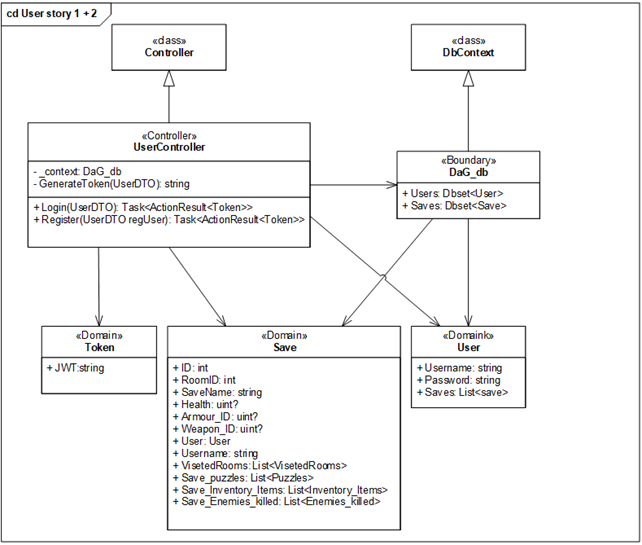
\includegraphics[width = \textwidth]{02-Body/Images/Backend_klasse_1_2.PNG}
\caption{Samlet klasse diagram over User story 1 og 2}
\label{fig:Design-Backend-Klasse-1-2}
\end{figure}

\noindent SaveControlleren har til ansvar at gemme og hente spil. Et klasse diagram for dennes håndtering af User Story 15,17 og 18 kan ses på \autoref{fig:Design-Backend-Sekvens-15-17-18}.\\


\begin{figure}[H]
\centering
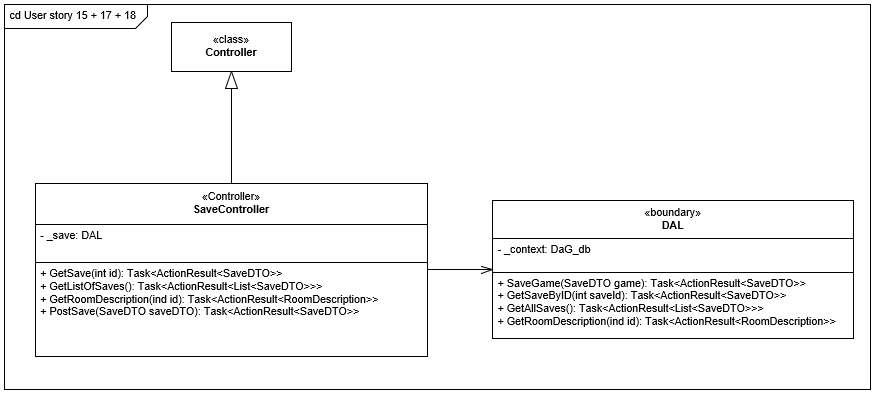
\includegraphics[width = \textwidth]{02-Body/Images/Backend_klasse_15_17_18.PNG}
\caption{Samlet klasse diagram for User story 15, 17 og 18}
\label{fig:Design-Backend-Sekvens-15-17-18}
\end{figure}

\noindent En fuld applikationsmodel over UserController og SaveControllers håndtering af de relevante User Stories kan ses i \textbf{Teknisk bilag afsnit 8.5}.\\

Backenden er blevet designet til at stille authentication/authorization til rådighed igennem, JWT. Derudover er der blevet opstillet de nødvendige routes for udførelsen af User Stories, som er blevet fundet igennem applikationsmodeller. BackendControlleren klassen er blevet introduceret på clienten, som står for HTTP request/response.\\ 


\newpage
